%!TEX root = ../rapport.tex

\chapter{Résultats} % (fold)
\label{cha:r_sultats}
Ce chapitre a pour but d'illustrer les résultats obtenus sur l'\emph{\gls{ipad}} par des maquettes qui sont tirées de l'application finale. Ce chapitre peut également servir de guide pour un utilisateur voulant utiliser l'application.

\section{Icône} % (fold)
\label{sec:ic_ne}
La figure \ref{gra:res01} montre l'îcone de l'application \emph{iGreenControl}. L'utilisateur presse sur cette îcone pour lancer l'application.
\begin{figure}[H]
     	\centering
     	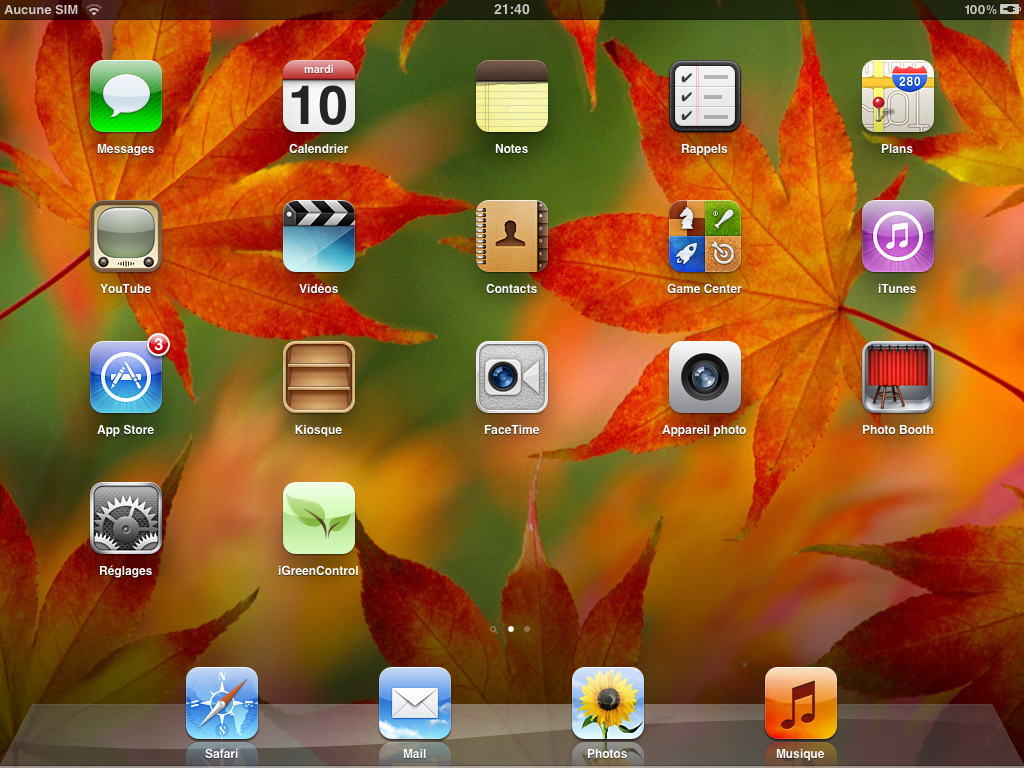
\includegraphics[width=14cm]{00_media/07_01.PNG}
     	\caption{Résultats - Icône}
     	\label{gra:res01}
 \end{figure} 
% section ic_ne (end)

\clearpage

\section{Login} % (fold)
\label{sec:login}
La figure \ref{gra:res02} illustre ce que voit l'utilisateur quand il lance l'application, il peut alors entrer ses informations d'authentification.
\begin{figure}[H]
     	\centering
     	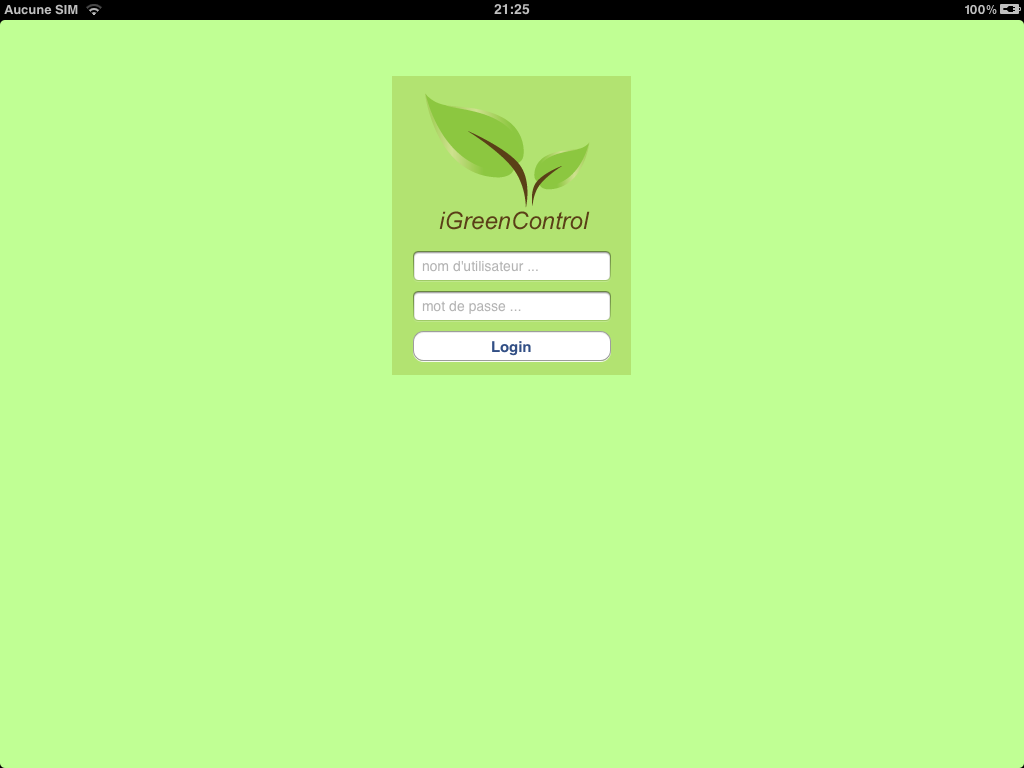
\includegraphics[width=\textwidth]{00_media/07_02.PNG}
     	\caption{Résultats - Ecran de login}
     	\label{gra:res02}
 \end{figure} 

\clearpage

\section{Informations} % (fold)
\label{sec:informations}
La figure \ref{gra:res03} résulte de la partie \emph{Infos} de l'application lorsque l'utilisateur clique sur le bouton correspondant.
\begin{figure}[H]
     	\centering
     	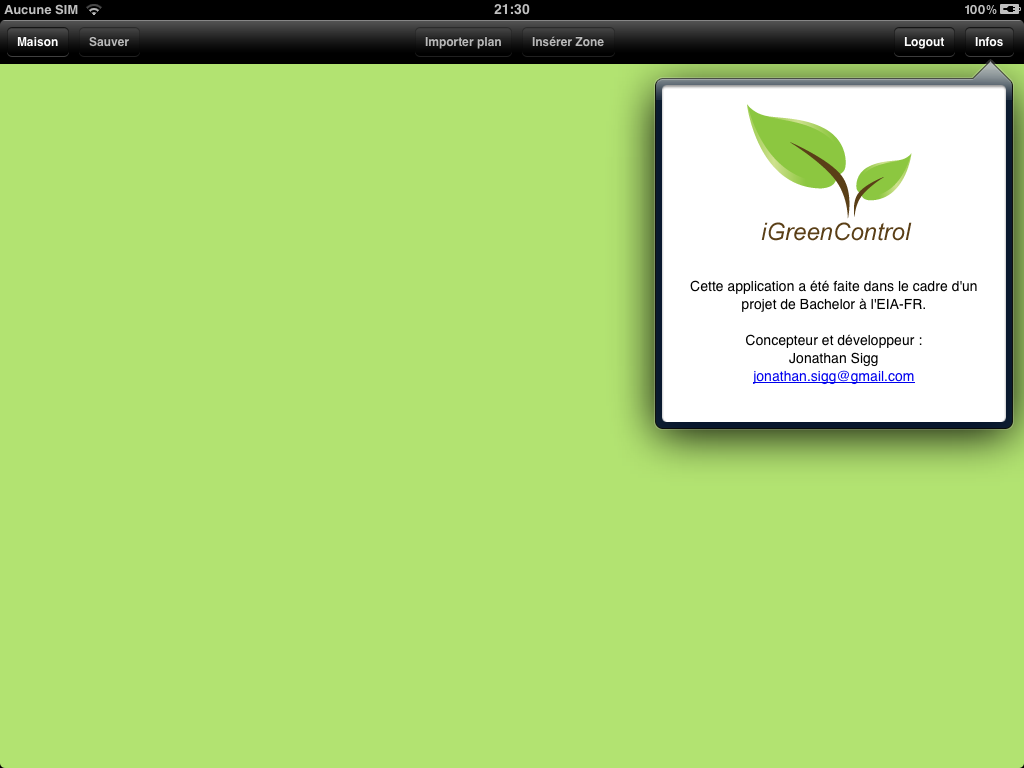
\includegraphics[width=\textwidth]{00_media/07_03.PNG}
     	\caption{Résultats - Informations}
     	\label{gra:res03}
 \end{figure} 

\clearpage


\section{Menu maison} % (fold)
\label{sec:menu_maisons}
La figure \ref{gra:res04} montre le menu qui apparait lorsque l'utilisateur clique sur le bouton \emph{Maison}. 

\begin{figure}[H]
    	\centering
    	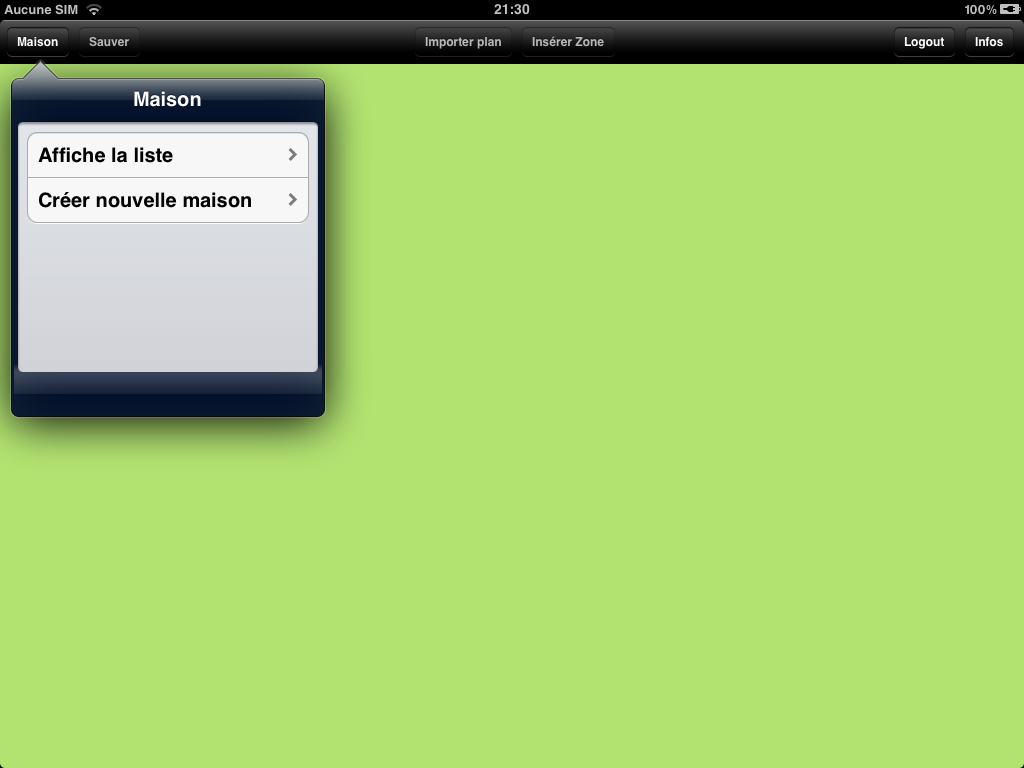
\includegraphics[width=\textwidth]{00_media/07_04.PNG}
    	\caption{Résultats - Menu maison}
    	\label{gra:res04}
\end{figure}

\clearpage


\section{Liste des maisons} % (fold)
\label{sub:liste_des_maisons}
Lorsque l'utilisateur clique sur la liste des maisons, il voit assez logiquement la liste des maisons qui lui appartiennent comme le montre la figure \ref{gra:res05}. Il peut alors soit cliquer sur une maison pour l'ouvrir, soit faire un défilement de gauche à droite avec le doigt pour afficher le bouton de suppression.
\begin{figure}[H]
        \centering
        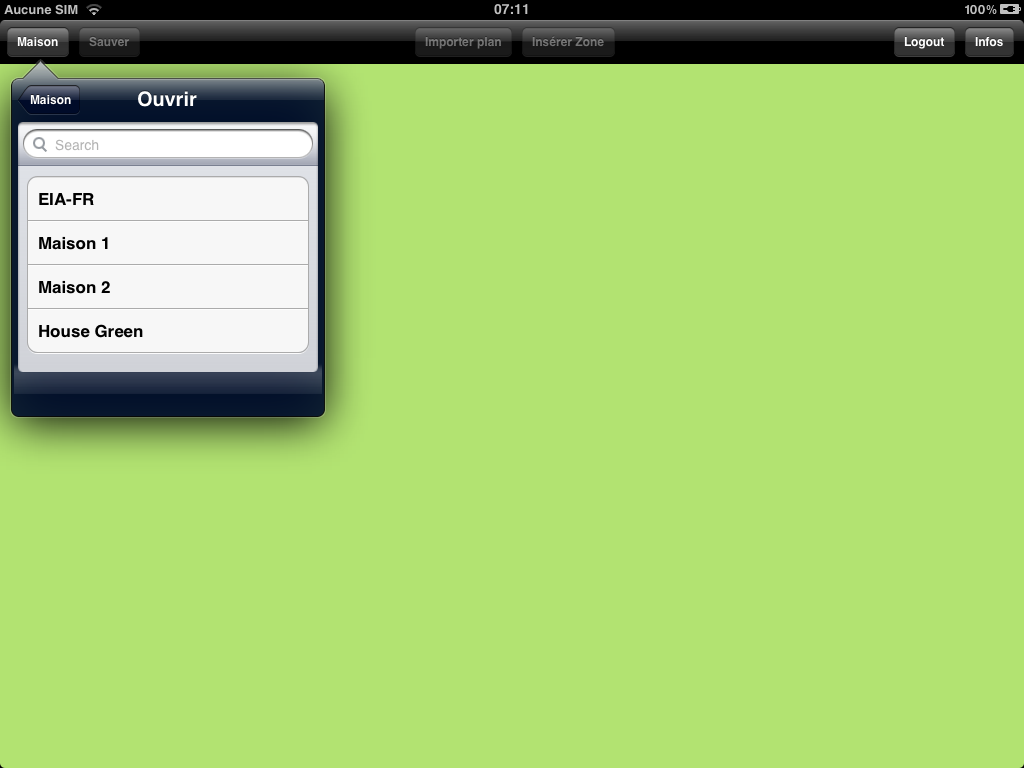
\includegraphics[width=\textwidth]{00_media/07_05.PNG}
        \caption{Résultats - Liste des maisons}
        \label{gra:res05}
\end{figure}
% subsection liste_des_maisons (end)

\clearpage


\section{Nouvelle maison} % (fold)
\label{sub:nouvelle_maison}
Lorsque l'utilisateur veut créer une nouvelle maison, il peut apercevoir un écran comme sur la figure \ref{gra:res06}. Il a la possibilité de remplir les informations et de créer la maison.
\begin{figure}[H]
        \centering
        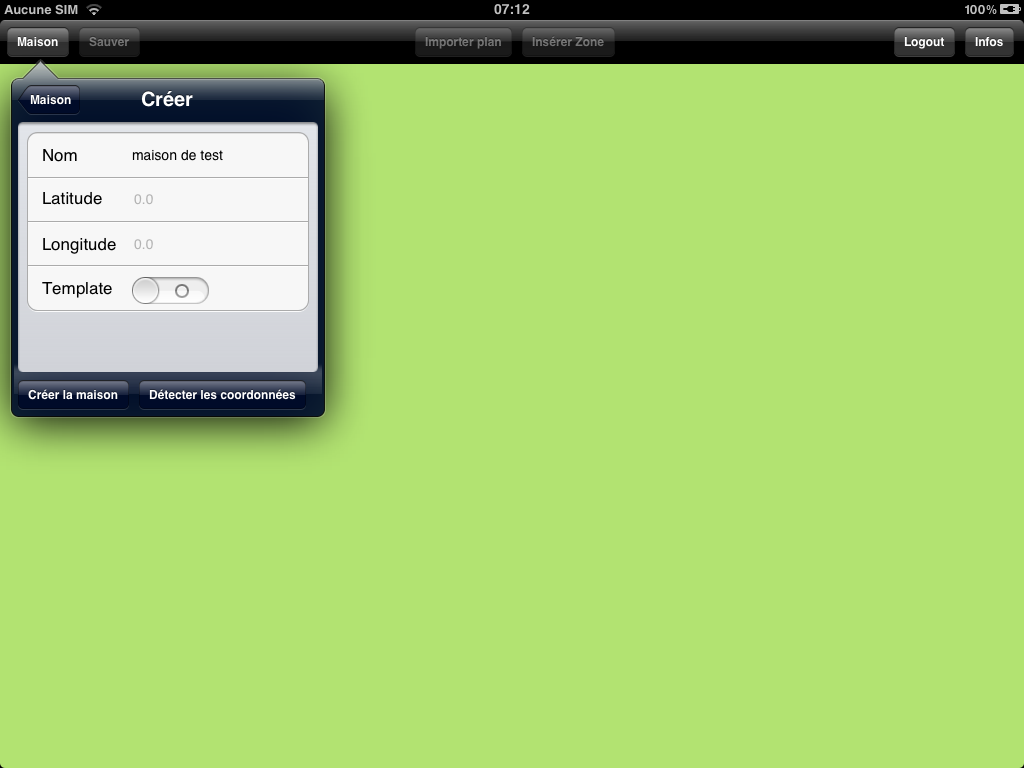
\includegraphics[width=\textwidth]{00_media/07_06.PNG}
        \caption{Résultats - Créer une nouvelle maison}
        \label{gra:res06}
\end{figure}

\clearpage


\section{Sélectionner une image} % (fold)
\label{sub:s_lectionner_une_image}
La figure \ref{gra:res07} montre l'explorateur d'image quand l'utilisateur veut importer un plan. Dès qu'une image est sélectionnée, celle-ci s'affiche dans l'application.
\begin{figure}[H]
        \centering
        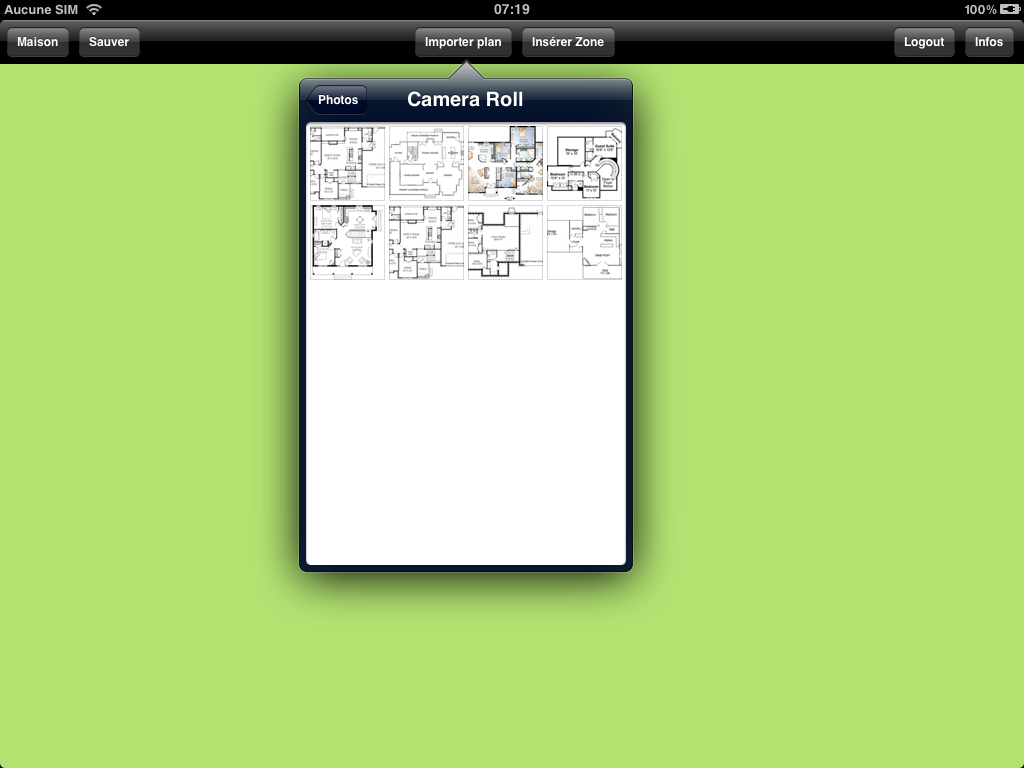
\includegraphics[width=\textwidth]{00_media/07_07.PNG}
        \caption{Résultats - Sélectionner une photo}
        \label{gra:res07}
\end{figure}

% subsection s_lectionner_une_image (end)

\clearpage


\section{Insertion d'une zone} % (fold)
\label{sub:insertion_d_une_zone}
La figure \ref{gra:res08} montre l'écran que voit l'utilisateur lorsqu'il désire insérer une nouvelle zone dans le plan. Il peut alors insérer les informations sur la zone et la créer en cliquand sur le bouton.
% subsection insertion_d_une_zone (end)
\begin{figure}[H]
        \centering
        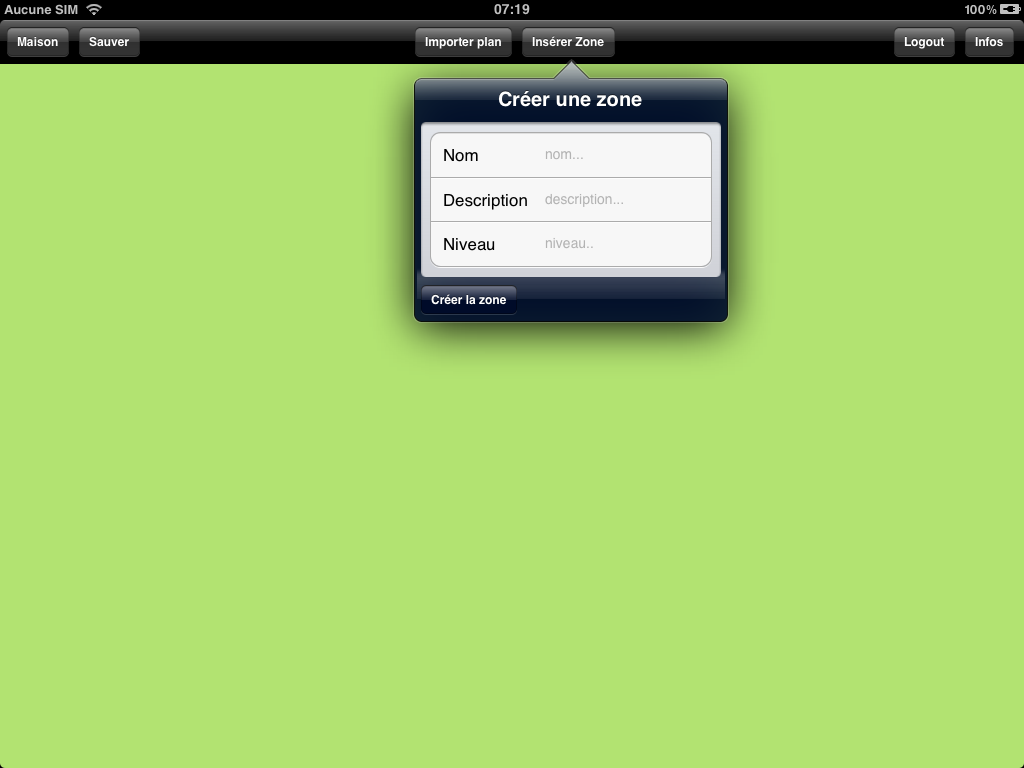
\includegraphics[width=\textwidth]{00_media/07_08.PNG}
        \caption{Résultats - Créer une nouvelle zone}
        \label{gra:res08}
\end{figure}

\clearpage


\section{Affichage d'un plan} % (fold)
\label{sub:subsection_ame}
Lorsque l'utilisateur ouvre une maison qui est déjà configurée et qui contient des zones et des capteurs, il peut par exemple voir un résultat comme sur la figure \ref{gra:res09}.

\medskip

Les opérations possibles pour le plan sont : 

\medskip

\begin{itemize}
    \item Redimensionner le plan (cela redimensionne également les éléments qui sont à l'intérieur du plan)
    \item Déplacer le plan (cela déplace également les éléments qui sont à l'intérieur du plan)
\end{itemize}

\medskip

Les opérations disponibles sur les zones sont : 

\medskip

\begin{itemize}
    \item Redimensionner uniquement les zones
    \item Déplacer les zones (cela déplace également les éventuels capteurs qui sont à l'intérieur)
    \item Faire pivoter les zones
    \item Presser un certain temps sur la zone afin d'afficher un menu spécifique à la zone
\end{itemize}

% subsection subsection_name (end)
\begin{figure}[H]
        \centering
        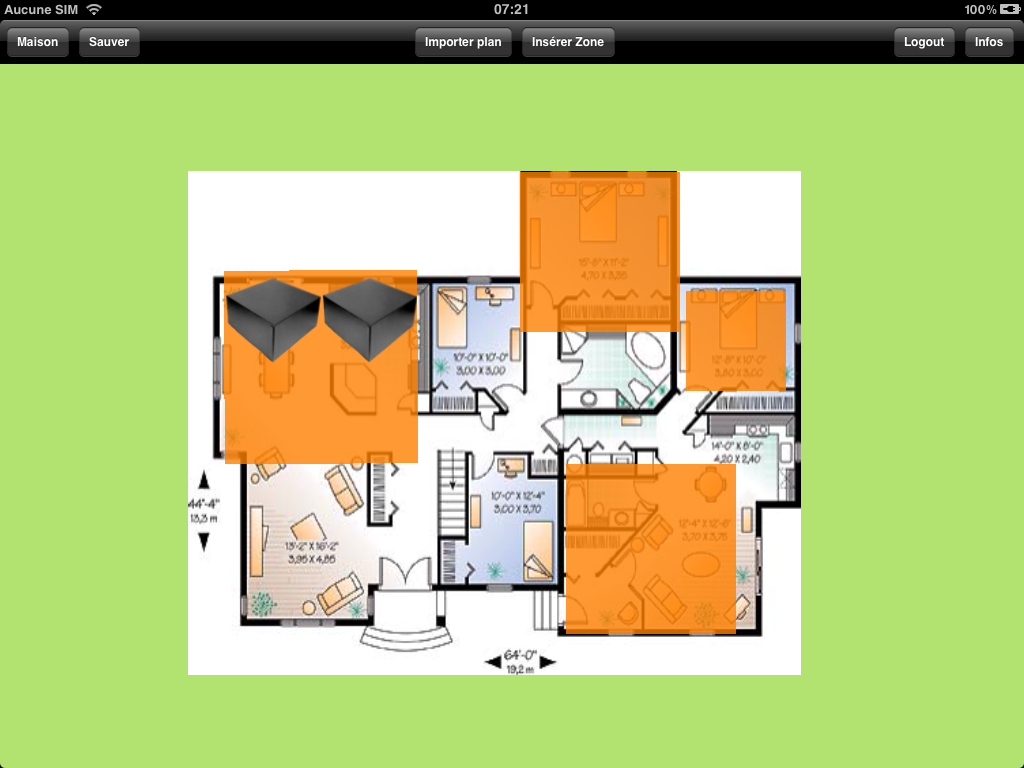
\includegraphics[width=\textwidth]{00_media/07_09.PNG}
        \caption{Résultats - Plan affiché}
        \label{gra:res09}
\end{figure}

\clearpage

\section{Paramètres d'une zone} % (fold)
\label{sub:param_tres_d_une_zone}
La figure \ref{gra:res10} montre le menu qui est présenté à l'utilisateur lorsque ce dernier presse un certain temps sur une zone. Il peut alors modifier les paramètres de la zone ou la supprimer.

\begin{figure}[H]
        \centering
        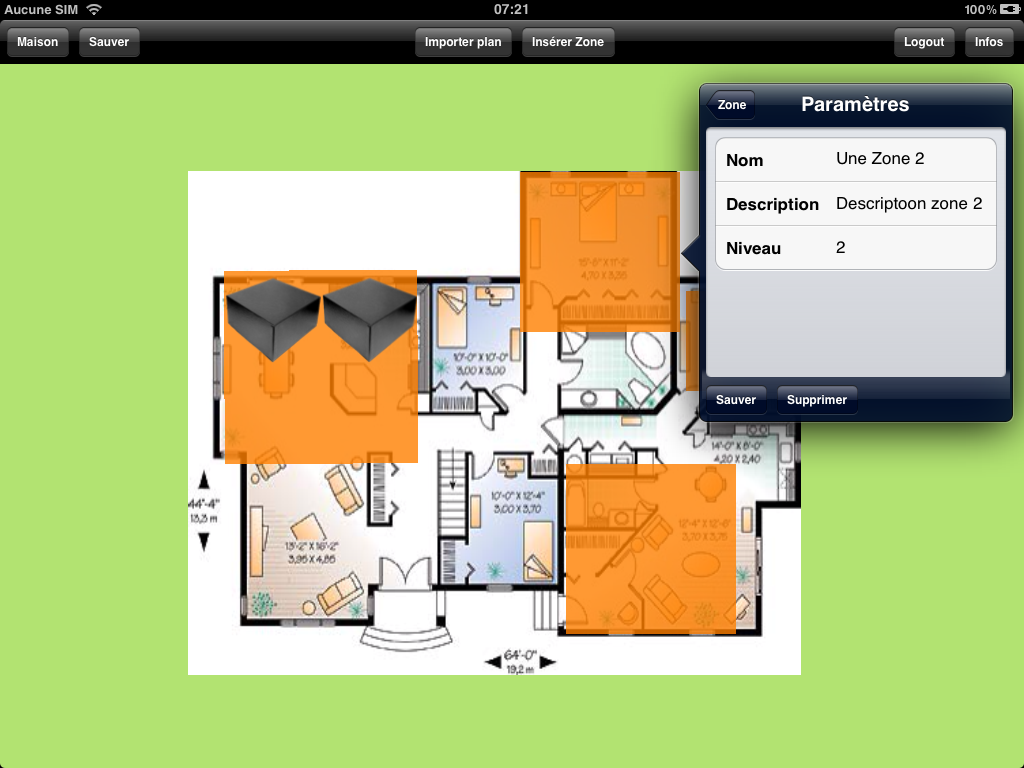
\includegraphics[width=\textwidth]{00_media/07_10.PNG}
        \caption{Résultats - Paramètres d'une zone}
        \label{gra:res10}
\end{figure}

\clearpage


\section{Insertion d'un capteur} % (fold)
\label{sub:insertion_d_un_capteur}

Toujours en pressant un certain temps sur une zone, l'utilisateur à la possibilité d'insérer un capteur. Une liste de capteurs disponible lui est alors présenté et il peut alors en sélectionner un dans le but de le relier à la zone. La liste des capteurs peut être aperçue à la figure \ref{gra:res11}.

\begin{figure}[H]
        \centering
        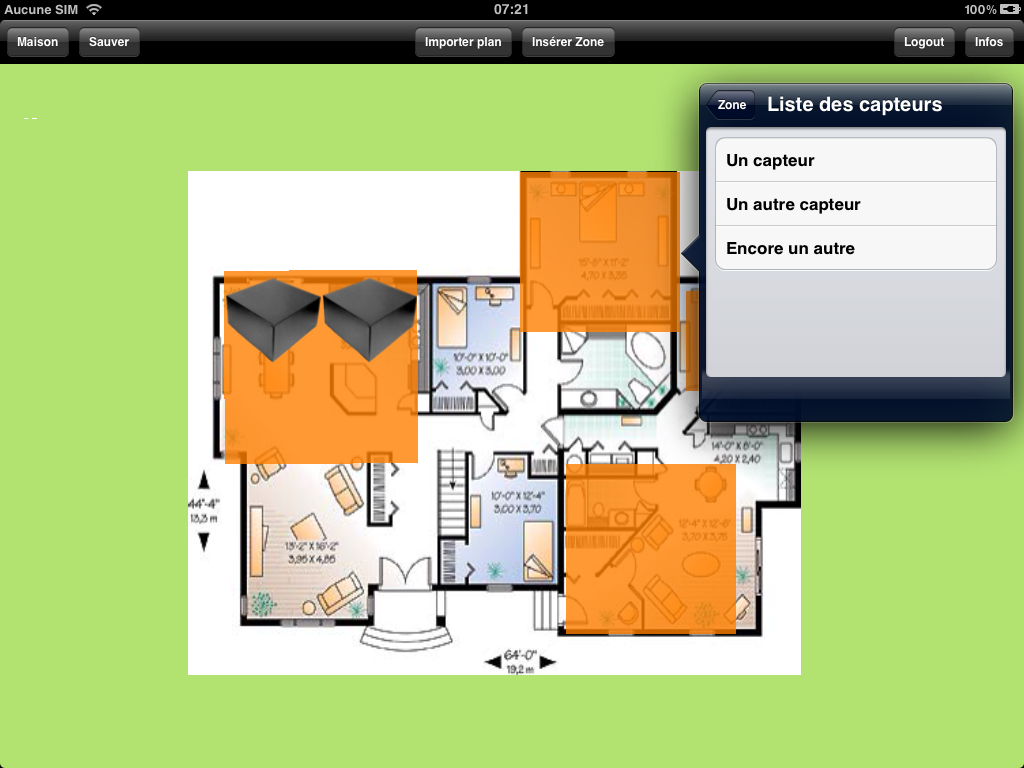
\includegraphics[width=\textwidth]{00_media/07_11.PNG}
        \caption{Résultats - Insertion d'un nouveau capteur}
        \label{gra:res11}
\end{figure}

\clearpage


\section{Paramètres d'un capteur} % (fold)
\label{sec:param_tres_d_un_capteur}
Lorsqu'il clique un certain temps sur un capteur, l'utilisateur voit apparaître un menu pour le capteur. Sur la figure \ref{gra:res12}, vous pouvez voir comment on peut modifier ou supprimer un capteur.

\begin{figure}[H]
        \centering
        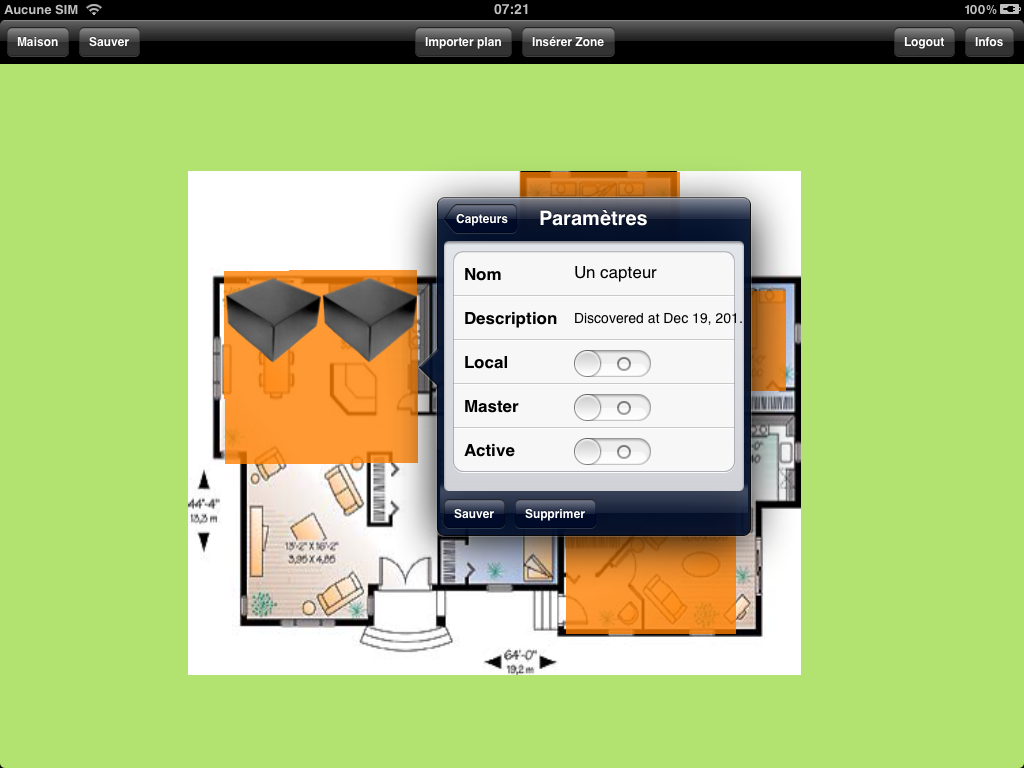
\includegraphics[width=\textwidth]{00_media/07_12.PNG}
        \caption{Résultats - Paramètres d'un capteur}
        \label{gra:res12}
\end{figure}

\clearpage


\section{Données d'un capteur} % (fold)
\label{sec:donn_es_d_un_capteur}
Sur la figure \ref{gra:res13}, ce sont les données du capteurs qui peuvent être distinguées. L'utilisateur peut alors les rafraîchir dès qu'il le souhaite.
% section donn_es_d_un_capteur (end)
\begin{figure}[H]
        \centering
        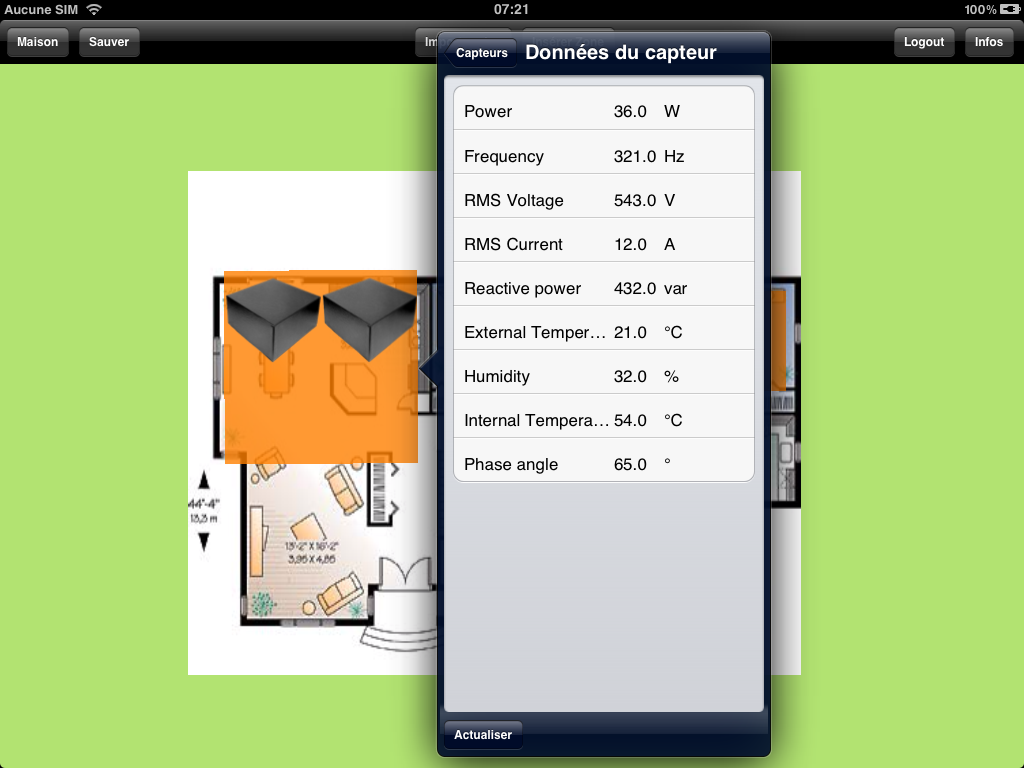
\includegraphics[width=\textwidth]{00_media/07_13.PNG}
        \caption{Résultats - Visualiser les données d'un capteur}
        \label{gra:res13}
\end{figure}
% subsection nouvelle_maison (end)
% section menu_maisons (end)

% section informations (end)
% chapter r_sultats (end)